\chapter{Data Validation Plots for $K_S^0$}

\begin{figure}[H]
	\caption{The distribution of variables used in KsFinder classification. The variables abbreviation can be referenced from Table III. The yellow solid lines are $K_S^0$ from data without KsFinder, and red solid lines are $K_S^0$ with KsFinder using MC13a for training.  The black dashed lines are $K_S^0$ with KsFinder using MC12b (run-dependent). Blue histogram is from MC13a without KsFinder and cyan histogram is from MC13a with KsFinder.}
\begin{subfigure}{0.5\linewidth}
	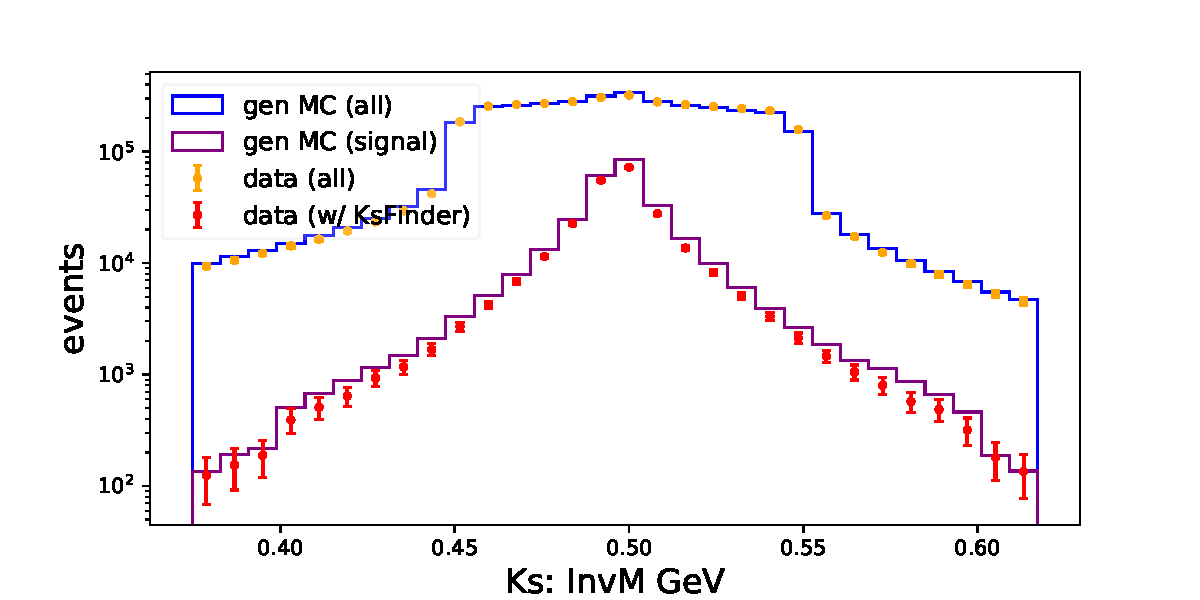
\includegraphics[page=1,height=4cm]{dataVarsPlot_Ks.pdf}
\end{subfigure}
\begin{subfigure}{0.5\linewidth}
		\includegraphics[page=2,height=4cm]{dataVarsPlot_Ks.pdf}
\end{subfigure}
\begin{subfigure}{0.5\linewidth}
		\includegraphics[page=3,height=4cm]{dataVarsPlot_Ks.pdf}
\end{subfigure}
\begin{subfigure}{0.5\linewidth}
		\includegraphics[page=4,height=4cm]{dataVarsPlot_Ks.pdf}
\end{subfigure}
\begin{subfigure}{0.5\linewidth}
		\includegraphics[page=5,height=4cm]{dataVarsPlot_Ks.pdf}
\end{subfigure}
\begin{subfigure}{0.5\linewidth}
	\includegraphics[page=6,height=4cm]{dataVarsPlot_Ks.pdf}
\end{subfigure}
\end{figure}
\begin{figure}[H]
\ContinuedFloat
\begin{subfigure}{0.5\linewidth}
	\includegraphics[page=7,height=4cm]{dataVarsPlot_Ks.pdf}
\end{subfigure}
\begin{subfigure}{0.5\linewidth}
	\includegraphics[page=8,height=4cm]{dataVarsPlot_Ks.pdf}
\end{subfigure}
\begin{subfigure}{0.5\linewidth}
	\includegraphics[page=9,height=4cm]{dataVarsPlot_Ks.pdf}
\end{subfigure}
\begin{subfigure}{0.5\linewidth}
	\includegraphics[page=10,height=4cm]{dataVarsPlot_Ks.pdf}
\end{subfigure}
\begin{subfigure}{0.5\linewidth}
	\includegraphics[page=11,height=4cm]{dataVarsPlot_Ks.pdf}
\end{subfigure}
\begin{subfigure}{0.5\linewidth}
	\includegraphics[page=12,height=4cm]{dataVarsPlot_Ks.pdf}
\end{subfigure}
\begin{subfigure}{0.5\linewidth}
	\includegraphics[page=13,height=4cm]{dataVarsPlot_Ks.pdf}
\end{subfigure}
\begin{subfigure}{0.5\linewidth}
	\includegraphics[page=14,height=4cm]{dataVarsPlot_Ks.pdf}
\end{subfigure}
\begin{subfigure}{0.5\linewidth}
	\includegraphics[page=15,height=4cm]{dataVarsPlot_Ks.pdf}
\end{subfigure}
\begin{subfigure}{0.5\linewidth}
	\includegraphics[page=16,height=4cm]{dataVarsPlot_Ks.pdf}
\end{subfigure}
\end{figure}

\begin{figure}[H]
\begin{subfigure}{0.5\linewidth}
	\includegraphics[page=17,height=4cm]{dataVarsPlot_Ks.pdf}
\end{subfigure}
\begin{subfigure}{0.5\linewidth}
	\includegraphics[page=18,height=4cm]{dataVarsPlot_Ks.pdf}
\end{subfigure}
\begin{subfigure}{0.5\linewidth}
	\includegraphics[page=19,height=4cm]{dataVarsPlot_Ks.pdf}
\end{subfigure}
\begin{subfigure}{0.5\linewidth}
	\includegraphics[page=22,height=4cm]{dataVarsPlot_Ks.pdf}
\end{subfigure}
\begin{subfigure}{0.5\linewidth}
	\includegraphics[page=23,height=4cm]{dataVarsPlot_Ks.pdf}
\end{subfigure}
\begin{subfigure}{0.5\linewidth}
	\includegraphics[page=24,height=4cm]{dataVarsPlot_Ks.pdf}
\end{subfigure}
\begin{subfigure}{0.5\linewidth}
	\includegraphics[page=25,height=4cm]{dataVarsPlot_Ks.pdf}
\end{subfigure}
\begin{subfigure}{0.5\linewidth}
	\includegraphics[page=26,height=4cm]{dataVarsPlot_Ks.pdf}
\end{subfigure}
\begin{subfigure}{0.5\linewidth}
	\includegraphics[page=27,height=4cm]{dataVarsPlot_Ks.pdf}
\end{subfigure}
	
\end{figure}